% !TeX root = ../main.tex
% Add the above to each chapter to make compiling the PDF easier in some editors.

\chapter{Gradient Descent}

Gradient descent\index{gradient descent} is a method for solving minimization problems such as \cref{eq:optimization_problem}, where we write $\s{\vx} \in \argmin_{\vx \in \sS} f(\vx)$. We say that a solution $\vx_k$ is \emph{$\epsilon$-approximate}\index{approximate solution} iff $f(\vx_k) - f(\s{\vx}) \leq \epsilon$ for some $\epsilon > 0$. For this chapter, we assume that the optimization problem is unconstrained, i.e., $\sS = \R^n$. The idea of gradient descent is to iteratively take a step in the opposite direction of the gradient starting from some initial point $\vx_0 \in \R^n$, \begin{align}
    \vx_{i+1} \gets \vx_i - \alpha \grad f(\vx_i),
\end{align} where $\alpha > 0$ is some learning rate.
\begin{marginfigure}
TBD
% \centering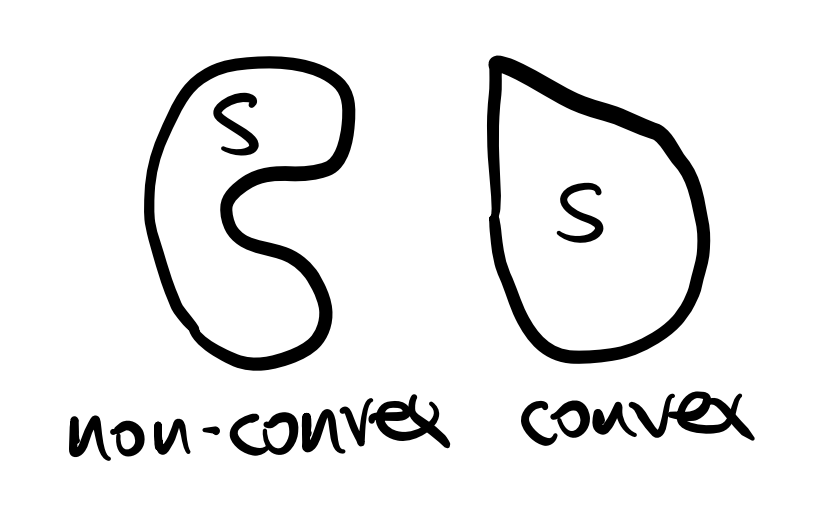
\includegraphics[width=4cm]{notes/figures/convex_set.png}
\caption{Non-convex function.}
\end{marginfigure}

When does gradient descent work? Clearly, we need that $f$ is convex, otherwise gradient descent might not converge to the global minimum at all. But this is not enough! We also need to ensure that the gradient of $f$ does not change arbitrarily when making very small steps, else the gradient direction would not be useful for us. This property is often called \emph{smoothness}.

\begin{marginfigure}
TBD
% \centering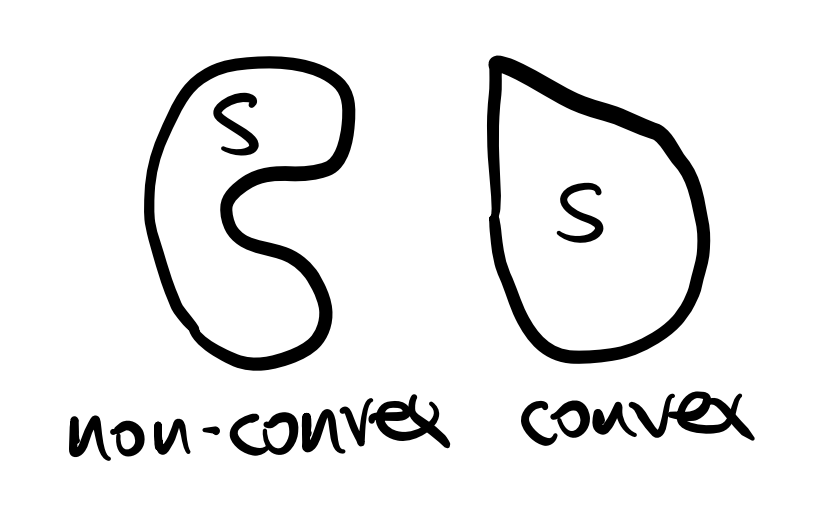
\includegraphics[width=4cm]{notes/figures/convex_set.png}
\caption{Function whose gradient is close to zero at a non-optimal point.}
\end{marginfigure}
Finally, it is intuitively clear that we can do much better when we can ensure that the gradient of $f$ is only close to zero around its minimum. If not, that is, we (almost) have ``saddle points'', the step size of gradient descent will slow down and depending on the stopping criterion we might even return a point that is not the minimizer. To exclude such functions from our analysis, we often assume that $f$ satisfies the \emph{PL condition}, or else is \emph{strongly convex}.

You can think of smoothness as providing a quadratic upper bound to our function, whereas strong convexity provides a quadratic lower bound.

\section{Smoothness}

\begin{defn}[Smoothness] Let $f: \sS \to \R$ be continuously differentiable. We say, $f$ is \emph{$\beta$-smooth}\index{smoothness} iff for any $\vx, \vy \in \sS$ \begin{align}
    \norm{\grad f(\vx) - \grad f(\vy)}_2 \leq \beta \norm{\vx - \vy}_2.
\end{align} In other words, the gradient of $f$ is $\beta$-Lipschitz.
\end{defn}
\begin{lem}
A twice continuously differentiable function $f: \sS \to \R$ is $\beta$-smooth iff for any $\vx \in \sS$, $\lambda_{\max}(\mH_f(\vx)) \leq \beta$.
\end{lem}
\begin{proof}
TBD
\end{proof}
\begin{lem}
A continuously differentiable function $f: \sS \to \R$ is $\beta$-smooth iff for any $\vx, \vy \in \sS$, \begin{align}
    f(\vy) \leq f(\vx) + \trans{\grad f(\vx)}(\vy - \vx) + \frac{\beta}{2}\norm{\vy - \vx}_2^2.
\end{align}
\end{lem} In words, $f(\vy)$ is upper bounded by a quadratic approximation based at $f(\vx)$.
\begin{proof}
TBD
\end{proof}

\subsection{Analysis of Gradient Descent}

A natural approach is to choose the gradient step of each iteration such that we minimize the upper bound (due to smoothness) based at the current solution, \begin{align}
    \grad_\vdelta \parentheses*{f(\vx_i) + \trans{\grad f(\vx_i)}\vdelta + \frac{\beta}{2}\norm{\vdelta}_2^2} = \grad f(\vx_i) + \beta\vdelta \overset{!}{=} 0,
\end{align} which is achieved for $\vdelta = -\frac{1}{\beta}\grad f(\vx_i)$. Thus, \begin{align}
    f(\vx_{i+1}) - f(\vx_i) &\leq \underbrace{\trans{\grad f(\vx_i)}\vdelta}_{-\frac{1}{\beta}\norm{\grad f(\vx_i)}_2^2} + \underbrace{\frac{\beta}{2}\norm{\vdelta}_2^2}_{\frac{1}{2\beta}\norm{\grad f(\vx_i)}_2^2} = -\frac{1}{2\beta}\norm{\grad f(\vx_i)}_2^2.
\end{align} Moreover, due to the first-order characterization of convexity, \begin{align}
    f(\vx_i) - f(\s{\vx}) \leq \trans{\grad f(\vx_i)}(\vx_i - \s{\vx}) \leq \norm{\grad f(\vx_i)}_2 \norm{\vx_i - \s{\vx}}_2,
\end{align} where the second inequality follows from Cauchy-Schwarz. Combining the previous two inequalities, \begin{align}
    f(\vx_{i+1}) - f(\vx_i) \leq -\frac{1}{2\beta}\parentheses*{\frac{f(\vx_i) - f(\s{\vx})}{\norm{\vx_i - \s{\vx}}_2}}^2 \leq -\frac{1}{2\beta}\parentheses*{\frac{f(\vx_i) - f(\s{\vx})}{\norm{\vx_0 - \s{\vx}}_2}}^2. \margintag{using that $\norm{\vx_i - \s{\vx}}_2 \leq \norm{\vx_0 - \s{\vx}}_2$, which follows from $f$ decreasing in every iteration and convexity} \label{eq:gd_gap}
\end{align}

\begin{thm}[Convergence of gradient descent] Suppose $f: \R^n \to \R$ is convex and $\beta$-smooth. The gradient descent scheme, \begin{align}
    \vx_{i+1} \defeq \vx_i - \frac{1}{\beta}\grad f(\vx_i),
\end{align} yields an $\epsilon$-approximate solution $\vx_k$ for some \begin{align*}
    k \geq \frac{2\beta\norm{\vx_0 - \s{\vx}}_2^2}{\epsilon}.
\end{align*}
\end{thm}

\begin{proof} We prove $f(\vx_k) - f(\s{\vx}) \leq \frac{2\beta\norm{\vx_0 - \s{\vx}}_2^2}{k+1}$ by induction on the length of the computation $k$. Suppose $k = 0$, then by the smoothness of $f$, \begin{align*}
    f(\vx_0) \leq f(\s{\vx}) - \underbrace{\trans{\grad f(\s{\vx})}}_{\vZero}(\vx_0 - \s{\vx}) + \frac{\beta}{2}\norm{\vx_0 - \s{\vx}}_2^2.
\end{align*} For the induction step, suppose that the statement holds for the $k$-th iterate. We write $\dgap_i \defeq f(\vx_i) - f(\s{\vx})$. Using \cref{eq:gd_gap}, \begin{align*}
    \dgap_{k+1} - \dgap_k \leq -\frac{\dgap_k^2}{2\beta\norm{\vx_0 - \s{\vx}}_2^2}.
\end{align*} Dividing by $\dgap_k \cdot \dgap_{k+1}$ and using that $\dgap_{k+1} > 0$ and $\dgap_k \geq \dgap_{k+1}$, we have, \begin{align*}
    \frac{1}{\dgap_k} - \frac{1}{\dgap_{k+1}} \leq -\frac{\dgap_k^2}{2\beta\norm{\vx_0 - \s{\vx}}_2^2 \dgap_k \dgap_{k+1}} \leq -\frac{1}{2\beta\norm{\vx_0 - \s{\vx}}_2^2}.
\end{align*} Thus, \begin{align*}
    \frac{1}{\dgap_{k+1}} \geq \frac{1}{2\beta\norm{\vx_0 - \s{\vx}}_2^2} + \frac{1}{\dgap_k} \geq \frac{(k+1) + 1}{2\beta\norm{\vx_0 - \s{\vx}}_2^2} \margintag{using the induction hypothesis} &\qedhere
\end{align*}
\end{proof}

\section{Strong Convexity}

We can improve our analysis, when we assume that $f$ is strongly convex, that is lower bounded by a quadratic. Intuitively, this ensures that our steps are large when we are far away from the optimum.

\begin{defn}[Strong convexity] Let $f: \sS \to \R$ be continuously differentiable. We say, $f$ is \emph{$\mu$-strongly convex}\index{strong convexity} iff for any $\vx,\vy \in \sS$, \begin{align}
    f(\vy) \geq f(\vx) + \trans{\grad f(\vx)}(\vy - \vx) + \frac{\mu}{2}\norm{\vy - \vx}_2^2.
\end{align}
\end{defn}
\begin{lem}
A twice continuously differentiable function $f: \sS \to \R$ is $\mu$-strongly convex iff for any $\vx \in \sS$, $\lambda_{\min}(\mH_f(\vx)) \geq \mu$.
\end{lem}
\begin{proof}
TBD
\end{proof}
\begin{cor}
If $f$ is $\beta$-smooth and $\mu$-strongly convex, then $\mu \leq \beta$.
\end{cor}

\begin{defn}[Condition number] We call $\kappa \defeq \frac{\beta}{\mu}$ the \emph{condition number}\index{condition number} of a function $f$ that is $\beta$-smooth and $\mu$-strongly convex.
\end{defn}

\subsection{Analysis of Gradient Descent}

\begin{thm}[Convergence of gradient descent with a strongly convex objective] Suppose $f: \R^n \to \R$ is $\mu$-strongly convex and $\beta$-smooth. The gradient descent scheme, \begin{align}
    \vx_{i+1} \defeq \vx_i - \frac{1}{\beta}\grad f(\vx_i),
\end{align} yields an $\epsilon$-approximate solution $\vx_k$ for some \begin{align*}
    k \geq \kappa\log\parentheses*{\frac{\beta\norm{\vx_0 - \s{\vx}}_2^2}{2\epsilon}}.
\end{align*}
\end{thm}
\begin{proof}
See the first graded homework.
\end{proof}

\section{Acceleration}

We can get an algorithm that converges substantially faster than vanilla gradient descent, using a method known as \emph{accelerated gradient descent}\index{accelerated gradient descent}. The key idea is to --- instead of only tracking the upper bound that is due to smoothness --- also use track lower bounds. In one iteration we might not make much progress in terms of reducing the upper bound (that is, improving our current solution), but instead increase the upper bound, which still reduces the error.

\begin{thm}[Convergence of accelerated gradient descent] Suppose $f: \R^n \to \R$ is convex and $\beta$-smooth. The accelerated gradient descent scheme, \begin{align}\begin{split}
    a_i &\defeq \frac{i+1}{2}, \quad A_i \defeq \frac{(i+1)(i+2)}{4} \\
    \vv_0 &\defeq \vx_0 - \frac{1}{2\beta} \grad f(\vx_0) \\
    \vy_i &\defeq \vx_i - \frac{1}{\beta} \grad f(\vx_i) \\
    \vx_{i+1} &\defeq \frac{A_i\vy_i + a_{i+1}\vv_i}{A_{i+1}} \\
    \vv_{i+1} &\defeq \vv_i - \frac{a_{i+1}}{\beta} \grad f(\vx_{i+1}),
\end{split}\end{align} yields an $\epsilon$-approximate solution $\vx_k$ for some \begin{align*}
    k \geq \sqrt{\frac{2\beta\norm{\vx_0 - \s{\vx}}_2^2}{\epsilon}}.
\end{align*}
\end{thm} Here, $\vy_i$ is the current solution (i.e., an upper bound), $\vv_i$ is a lower bound, and $\vx_i$ a point that trades improving the lower/upper bounds.

\begin{proof}
TBD
\end{proof}

\subsection{Acceleration with Strongly Convex Objectives}

\begin{thm}[Convergence of accelerated gradient descent with a strongly convex objective] Suppose $f: \R^n \to \R$ is $\mu$-strongly convex and $\beta$-smooth. The accelerated gradient descent scheme, \begin{align}\begin{split}
    \vy_0 &\defeq \vx_0 \\
    \vy_{i+1} &\defeq \vx_i - \frac{1}{\beta} \grad f(\vx_i) \\
    \vx_{i+1} &\defeq (1+\theta)\vy_{i+1} + \theta\vy_i
\end{split}\end{align} for $\theta \defeq \frac{\sqrt{\kappa} - 1}{\sqrt{\kappa} + 1}$ yields an $\epsilon$-approximate solution $\vx_k$ for some \begin{align*}
    k \geq \sqrt{\kappa}\log\parentheses*{\frac{\beta\norm{\vx_0 - \s{\vx}}_2^2}{\epsilon}}.
\end{align*}
\end{thm}
\begin{proof}
See the first graded homework.
\end{proof}
